\documentclass[conference]{IEEEtran}
\IEEEoverridecommandlockouts
\usepackage{cite}
\usepackage{balance}
\usepackage{amsmath,amssymb,amsfonts}
\usepackage{graphicx}
\usepackage{textcomp}
\usepackage{xcolor}
\usepackage{booktabs}
\usepackage{array}
\usepackage{tikz}
\usetikzlibrary{positioning,arrows.meta,fit,calc}
\usepackage{algorithm}
\usepackage{algorithmic}
\usepackage[hidelinks]{hyperref}
\newcommand{\PolCases}{16,032}
\newcommand{\PolViol}{0}
\newcommand{\PolAuto}{401}
\newcommand{\PolReview}{3,607}
\newcommand{\PolMonitor}{4,000}
\newcommand{\PolOverride}{8,008}
\newcommand{\PolUnavail}{16}
\newcommand{\PolAutoUnhealthy}{0}
\newcommand{\PolMs}{42}
\newcommand{\EtoECases}{32,032}
\newcommand{\EtoEViolBefore}{2,807}
\newcommand{\EtoEViolAfter}{0}
\newcommand{\EtoEFiredBefore}{9,624}
\newcommand{\EtoEFiredAfter}{6,817}
\newcommand{\DualN}{604}
\newcommand{\DualHold}{69.7}
\newcommand{\DualGap}{64.1}
\newcommand{\DualStraddle}{10.3}
\newcommand{\DualStraddleOnly}{5.6}
\newcommand{\DualEligible}{515}
\newcommand{\DualEligibleHeld}{76.9}
\newcommand{\DualBoth}{453}
\newcommand{\DualBothHeld}{73.7}
\newcommand{\DualMeanGap}{0.167}
\newcommand{\DualMaxGap}{0.347}
\newcommand{\DualRfAuto}{79.5}
\newcommand{\DualXgbAuto}{80.8}
\newcommand{\GuardCtx}{200}
\newcommand{\GuardFacts}{8.1}
\newcommand{\GuardMs}{2.1}
\newcommand{\GuardFalseRej}{0}
\newcommand{\BandCalm}{21}
\newcommand{\BandWatch}{8}
\newcommand{\BandAdmin}{10}
\newcommand{\BandAuto}{161}
\newcommand{\GProbSmallDeployed}{94.0}
\newcommand{\GProbSmallNoscale}{94.0}
\newcommand{\GProbSmallFactsonly}{95.0}
\newcommand{\GProbSmallStrict}{95.0}
\newcommand{\GProbLargeDeployed}{95.5}
\newcommand{\GProbLargeNoscale}{95.5}
\newcommand{\GProbLargeFactsonly}{96.5}
\newcommand{\GProbLargeStrict}{96.5}
\newcommand{\GRainDeployed}{97.0}
\newcommand{\GRainNoscale}{97.0}
\newcommand{\GRainFactsonly}{97.5}
\newcommand{\GRainStrict}{97.5}
\newcommand{\GRiverDeployed}{98.0}
\newcommand{\GRiverNoscale}{98.5}
\newcommand{\GRiverFactsonly}{98.0}
\newcommand{\GRiverStrict}{98.5}
\newcommand{\GCountDeployed}{97.5}
\newcommand{\GCountNoscale}{97.5}
\newcommand{\GCountFactsonly}{98.0}
\newcommand{\GCountStrict}{98.0}
\newcommand{\GEtaDeployed}{94.0}
\newcommand{\GEtaNoscale}{94.0}
\newcommand{\GEtaFactsonly}{95.0}
\newcommand{\GEtaStrict}{95.0}
\newcommand{\GWordsDeployed}{0.0}
\newcommand{\GWordsNoscale}{0.0}
\newcommand{\GWordsFactsonly}{0.0}
\newcommand{\GWordsStrict}{0.0}
\newcommand{\GAllDeployed}{96.0}
\newcommand{\GAllNoscale}{96.1}
\newcommand{\GAllFactsonly}{96.7}
\newcommand{\GAllStrict}{96.8}
\newcommand{\GMissDeployed}{4.0}
\newcommand{\GInjected}{1,200}
\newcommand{\GProbSmallTyped}{97.0}
\newcommand{\GProbLargeTyped}{97.0}
\newcommand{\GRainTyped}{100.0}
\newcommand{\GRiverTyped}{98.5}
\newcommand{\GCountTyped}{100.0}
\newcommand{\GEtaTyped}{100.0}
\newcommand{\GWordsTyped}{81.5}
\newcommand{\GAllTyped}{98.8}
\newcommand{\GTypedFalseRej}{0}
\newcommand{\GTypedMissN}{15}
\newcommand{\GTypedWordMiss}{37}
\newcommand{\DeltaStraddleOnly}{10.3}
\newcommand{\DeltaThirtyHold}{10.9}
\newcommand{\DeltaThirtyBoth}{0.2}
\newcommand{\GMissN}{48}
\newcommand{\GMissFact}{39}
\newcommand{\GMissRule}{8}
\newcommand{\GMissScale}{1}
\newcommand{\GMissEtaFact}{10}
\newcommand{\DeltaZeroBoth}{0.31}
\newcommand{\MissExProb}{87.3}
\newcommand{\MissExEta}{87}
\newcommand{\LiveJudN}{300}
\newcommand{\LiveJudNTwenty}{150}
\newcommand{\LiveJudNOneTwenty}{150}
\newcommand{\LiveN}{300}
\newcommand{\LiveStates}{150}
\newcommand{\LiveUnsup}{109}
\newcommand{\LiveUnsupPct}{36.3}
\newcommand{\LiveTwentyUnsupPct}{33.3}
\newcommand{\LiveOneTwentyUnsupPct}{39.3}
\newcommand{\LiveEta}{106}
\newcommand{\LiveEtaPct}{97}
\newcommand{\LiveOverrides}{4}
\newcommand{\LiveJudgeNone}{23}
\newcommand{\LiveDepRec}{89.0}
\newcommand{\LiveDepFpr}{5.8}
\newcommand{\LiveDepPrec}{89.8}
\newcommand{\LiveDepFp}{11}
\newcommand{\LiveTypRec}{93.6}
\newcommand{\LiveTypFpr}{10.5}
\newcommand{\LiveTypPrec}{83.6}
\newcommand{\LiveTypFp}{20}
\newcommand{\LiveJDepRec}{89.0}
\newcommand{\LiveJDepFpr}{5.8}
\newcommand{\LiveJTypRec}{93.6}
\newcommand{\LiveJTypFpr}{10.5}
\newcommand{\LiveJJudRec}{99.1}
\newcommand{\LiveJJudFpr}{14.1}
\newcommand{\LiveJUnsup}{109}
\newcommand{\LiveJJudMiss}{1}
\newcommand{\LiveDepMiss}{12}
\newcommand{\LiveDepMissWords}{5}
\newcommand{\LiveDepMissClock}{5}
\newcommand{\LiveTypFpN}{20}
\newcommand{\LiveOverclaim}{43}
\newcommand{\LiveOverclaimPct}{14}
\newcommand{\LiveDigitEtaCaught}{97}
\newcommand{\JudgeInjStates}{40}
\newcommand{\JudgeInjItems}{320}
\newcommand{\JudgeFalseRej}{0.0}
\newcommand{\JudgeFalseRejN}{0}
\newcommand{\JudgeInjNum}{97.1}
\newcommand{\JudgeProbSmallMiss}{15}
\newcommand{\JudgeInjWords}{90.0}
\newcommand{\DepInjNumSub}{96.7}
\newcommand{\TypInjNumSub}{99.2}
\newcommand{\JudgeModel}{Qwen3 (27B)}
\newcommand{\CalTest}{910}
\newcommand{\CalTrain}{3638}
\newcommand{\CalPos}{35.8}
\newcommand{\EceRf}{0.044}
\newcommand{\EceCalRf}{0.031}
\newcommand{\BrierRf}{0.163}
\newcommand{\MeanPRf}{0.379}
\newcommand{\EceXgb}{0.108}
\newcommand{\EceCalXgb}{0.018}
\newcommand{\BrierXgb}{0.182}
\newcommand{\MeanPXgb}{0.378}
\newcommand{\CalGapMean}{0.101}
\newcommand{\DeltaCv}{0.28}
\newcommand{\GateDepHold}{26.9}
\newcommand{\GateDepBoth}{29.1}
\newcommand{\GateDepErrHeld}{37.1}
\newcommand{\GateDepErrRel}{20.3}
\newcommand{\GateCvHold}{9.1}
\newcommand{\GateCvBoth}{2.2}
\newcommand{\GateCvErrHeld}{48.2}
\newcommand{\GateCvErrRel}{22.5}
\newcommand{\GateStHold}{7.6}
\newcommand{\GateStBoth}{0.0}
\newcommand{\GateStErrHeld}{52.2}
\newcommand{\GateStErrRel}{22.6}
\newcommand{\GateCalHold}{10.5}
\newcommand{\GateCalBoth}{7.0}
\newcommand{\GateDepErrRatio}{1.8}
\newcommand{\GateStErrRatio}{2.3}
\newcommand{\XgbHighConf}{0.84}
\newcommand{\XgbHighFreq}{0.67}
\newcommand{\DevDepRec}{89.0}
\newcommand{\DevDepFpr}{5.8}
\newcommand{\HoDepRec}{96.1}
\newcommand{\HoDepFpr}{7.1}
\newcommand{\HoDepFp}{4}
\newcommand{\HoDepMiss}{3}
\newcommand{\DevTypRec}{93.6}
\newcommand{\DevTypFpr}{10.5}
\newcommand{\HoTypRec}{100.0}
\newcommand{\HoTypFpr}{17.9}
\newcommand{\HoTypFp}{10}
\newcommand{\HoTypMiss}{0}
\newcommand{\DevVtwoRec}{100.0}
\newcommand{\DevVtwoFpr}{0.0}
\newcommand{\HoVtwoRec}{98.7}
\newcommand{\HoVtwoFpr}{12.5}
\newcommand{\HoVtwoFp}{7}
\newcommand{\HoVtwoMiss}{1}
\newcommand{\HoN}{132}
\newcommand{\HoStates}{150}
\newcommand{\HoUnsup}{76}
\newcommand{\HoUnsupPct}{57.6}
\newcommand{\HoParseFail}{18}
\newcommand{\HoCountPct}{64}
\newcommand{\HoOverrides}{8}
\newcommand{\VtwoUs}{371}
\newcommand{\VtwoInjGround}{0.0}
\newcommand{\VtwoInjNum}{98.8}
\newcommand{\VtwoInjWords}{81.5}
\newcommand{\ErrOssEtaMin}{32}
\newcommand{\ErrOssEtaMax}{39}
\newcommand{\ErrAllamEta}{4.5}
\newcommand{\ErrAllamQty}{39}
\newcommand{\ErrAllamProb}{16}


\begin{document}

\title{Rules Decide, Language Models Narrate:\\
A Fail-Closed Multi-Agent Architecture for\\
Flood Response with Numeric Grounding}

%<AUTHORS>
\author{
\IEEEauthorblockN{Nandhakumar T}
\IEEEauthorblockA{\textit{Department of Information Technology}\\
\textit{Sona College of Technology}\\
Salem, Tamil Nadu, India\\
nandhakumartm93@gmail.com}
\and
\IEEEauthorblockN{Balakarthikeyan B S}
\IEEEauthorblockA{\textit{Department of Artificial Intelligence and Data Science}\\
\textit{Sona College of Technology}\\
Salem, Tamil Nadu, India\\
balasan2626@gmail.com}
\and
\IEEEauthorblockN{Gowthaman J}
\IEEEauthorblockA{\textit{Department of Artificial Intelligence and Data Science}\\
\textit{Sona College of Technology}\\
Salem, Tamil Nadu, India\\
gowthamanjanadhran@gmail.com}
\and
\IEEEauthorblockN{Abhishek S}
\IEEEauthorblockA{\textit{Department of Artificial Intelligence and Data Science}\\
\textit{Sona College of Technology}\\
Salem, Tamil Nadu, India\\
abisheksengodan18@gmail.com}
}
%</AUTHORS>

\maketitle

\begin{abstract}
Large language models (LLMs) are proposed as the voice of emergency-management software, but they can state numbers that are not in the data. In our flood-response architecture, eleven agents share one state, a deterministic policy chooses every action and the LLM only narrates. Three mechanisms keep it fail-closed: a health-gated policy, a disagreement gate between two classifiers and a numeric guard that replaces any message with an unsupported number by a template. We evaluate all three on the deployed code. A composed check of the path from policy to dispatch found \EtoEViolBefore{} of \EtoECases{} cases in which teams were sent although the verified policy asked for review; after a one-line fix it found \EtoEViolAfter. Of \LiveN{} replies from two open-weight LLMs, \LiveUnsupPct\% contained an unsupported number, almost all invented arrival times. The deployed guard caught \LiveDepRec\% of these and a slot-typed guard \LiveTypRec\%, with false-rejection rates of \LiveDepFpr\% and \LiveTypFpr\%; an LLM judge caught all it checked but needs a model call per message and missed \JudgeProbSmallMiss\% of injected one-digit probability errors. A revised guard, frozen before a third model family was queried, caught \HoVtwoRec\% of unsupported replies from that model, but its false rejections rose to \HoVtwoFpr\%. On the classifiers' held-out data, held cases were wrong \GateDepErrRatio{} times as often as released ones, and holding only when the models straddle the threshold held a quarter as many cases while flagging errors more sharply. Fail-closed properties must be checked on the whole path to action, and narration against typed state.
\end{abstract}

\begin{IEEEkeywords}
large language models, hallucination, multi-agent systems, fail-safe design, flood response
\end{IEEEkeywords}

\section{Introduction}
During a flood, an emergency operations centre runs on short spoken messages: the river is at this level, the forecast says this, send a team there. Software that supports the centre is increasingly asked to \emph{speak}, and LLMs make this easy. They also produce confident statements that their input does not support \cite{Ji2023}. On an operations net a wrong number can trigger or cancel an evacuation.

Agentic systems let the model plan and call tools \cite{Yao2023,Schick2023,Wu2024}. For a safety-critical setting we take the opposite position: decisions are made by small deterministic agents whose behaviour can be checked exhaustively, and the LLM only turns their state into radio traffic. This follows the view that the level of automation should be chosen per function and per risk \cite{Parasuraman2000} and that safety is a property of the control structure rather than of one component \cite{Leveson2011}. Two questions remain open. Does the verified decision actually govern what the system does? And how often does the narrator misstate the state in practice, and which check catches it?

We answer both on an open flood decision-support prototype for the Delhi Yamuna corridor. Our contributions are:
\begin{enumerate}
\item An architecture in which agents share one state and event log, only deterministic agents can act, and generated text is advisory, with three fail-closed mechanisms defined formally.
\item A composed check of the path from observation to dispatch, which found that dispatch bypassed the verified policy in \EtoEViolBefore{} of \EtoECases{} cases and confirmed the fix.
\item A measurement of numeric grounding on \LiveN{} replies of two open-weight LLMs and on injected errors, comparing the deployed guard, a slot-typed guard and an LLM-as-judge baseline \cite{Zheng2023}, with a revised guard tested on a model family held out until the guard was frozen.
\item A held-out calibration study of the dual-model gate, which shows when model disagreement signals error and gives a tolerance set from training data alone.
\end{enumerate}

\section{Related Work}
\textit{Agents and agentic LLMs.} Software agents that perceive, decide and act have a long history \cite{Wooldridge1995}, and disaster response has been a multi-agent benchmark since RoboCup Rescue \cite{Kitano1999}. LLM agents interleave reasoning with actions \cite{Yao2023}, learn when to call tools \cite{Schick2023} and cooperate in conversations \cite{Wu2024}; surveys describe them as memory, planner and action interface around a model \cite{WangL2024}. Our agents keep memory and actions but take planning away from the model.

\textit{Hallucination detection and guardrails.} Generated text departs from its source in many ways \cite{Ji2023}. Retrieval grounds generation in documents \cite{Lewis2020}; post-hoc checkers decompose text into atomic claims \cite{Min2023}, sample the model several times \cite{Manakul2023}, let the model verify itself \cite{Dhuliawala2024} or ask another model to judge \cite{Zheng2023}. Programmable rails constrain dialogue flows \cite{Rebedea2023}, runtime verification checks outputs against expert specifications \cite{Zhang2025}, and runtime enforcement blocks unsafe agent actions \cite{WangH2026}. These methods are probabilistic, rely on further model calls, or check actions rather than reported values. Our facts are a handful of numbers in a known state, so a deterministic, typed check is possible.

\textit{Safe automation.} Levels of automation should fall where errors are costly \cite{Parasuraman2000}; run-time shields block unsafe actions of learned controllers \cite{Alshiekh2018}; and ensembles estimate uncertainty \cite{Dietterich2000,Lakshminarayanan2017}. We use disagreement between two classifiers as a hold signal instead of averaging them.

\textit{Research gap.} We found no study that measures, on the deployed code of an emergency system, both whether a verified decision governs actuation and how often real LLM narration misstates numeric state, nor one that compares deterministic and model-based checks of that narration.

\section{Architecture}
\label{sec:arch}
Fig.~\ref{fig:arch} shows the system. A FastAPI backend runs one pipeline per tick, in live mode (Open-Meteo weather and river data) or in simulation mode (a digital twin of the corridor). Eleven agents share one state object and write every event to a MongoDB log and a WebSocket stream, so the interface shows what each agent did and why. Table~\ref{tab:roles} lists their authority: only the Flood Risk agent's policy can start a response, and dispatch executes only what the policy allowed. Algorithm~\ref{alg:tick} gives one tick. The policy and the gate run before any planning agent, and narration runs last, after the decision is logged, so a narration failure can delay a radio message but cannot change a decision.

\begin{table}[t]
\caption{Agents, their events and their authority}
\label{tab:roles}
\centering
\footnotesize
\setlength{\tabcolsep}{2.0pt}
\begin{tabular}{lll}
\toprule
Agent & Emits & Authority\\
\midrule
Weather, Dam & rainfall, river and barrage stage & inform\\
Flood Risk & policy action $\pi$ and reason & \textbf{decide} (gated)\\
Traffic, Shelter & road risk; ranked shelters & inform, rank\\
Evacuation & candidate routes, plan & propose\\
Rescue & team dispatch & act after $\pi$\\
Ambulance, Disaster Team & radio turns & narrate\\
Administrator & hold notices, radio turns & hold, narrate\\
Card Monitor & sudden-change alerts & inform\\
\bottomrule
\end{tabular}
\end{table}

\begin{algorithm}[t]
\caption{One pipeline tick (after the fix)}
\label{alg:tick}
\begin{algorithmic}[1]
\small
\STATE read observations; Weather and Dam agents emit updates
\STATE $p_{\mathrm{RF}},p_{\mathrm{XGB}},p \leftarrow$ classifiers; $H\leftarrow$ (\ref{eq:dual})
\STATE $(h_d,h_m,h_s)\leftarrow$ health checks; $a\leftarrow\pi(p,\mathbf{h},o)$ by (\ref{eq:policy})
\STATE \textbf{if} $H$ \AND \NOT $o$ \textbf{then} $a\leftarrow\textsc{review}$ and log the hold reason
\STATE \textbf{if} $a\neq\textsc{monitor}$ \textbf{then} rank roads, shelters, routes
\STATE \textbf{if} $a\in\{\textsc{auto},\textsc{override}\}$ \AND band$(p)=$ auto \textbf{then} dispatch
\STATE $T\leftarrow$ LLM turns for band$(p)$; \textbf{if} \NOT $\Gamma(T)$ \textbf{then} $T\leftarrow$ template
\STATE broadcast state, decision and $T$
\end{algorithmic}
\end{algorithm}

\begin{figure}[t]
\centering
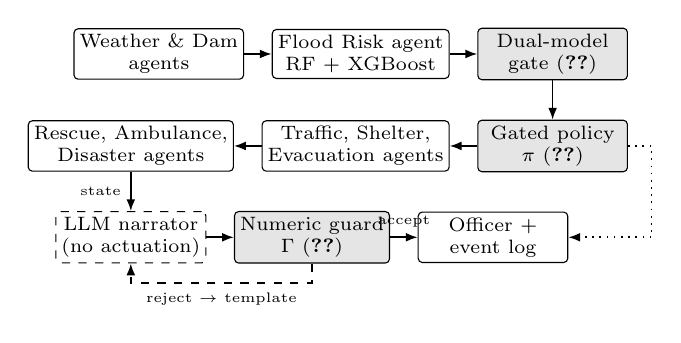
\begin{tikzpicture}[
  font=\scriptsize,
  box/.style={draw, rounded corners=1.5pt, align=center, minimum width=1.9cm, minimum height=0.58cm, inner sep=2pt},
  gate/.style={box, fill=gray!20},
  llm/.style={box, dashed},
  arr/.style={-{Latex[length=1.5mm]}, semithick}]
\node[box] (wx) {Weather \& Dam\\agents};
\node[box, right=0.35cm of wx] (fr) {Flood Risk agent\\RF + XGBoost};
\node[gate, right=0.35cm of fr] (dual) {Dual-model\\gate (\ref{eq:dual})};
\node[gate, below=0.5cm of dual] (pol) {Gated policy\\$\pi$ (\ref{eq:policy})};
\node[box, left=0.35cm of pol] (ops) {Traffic, Shelter,\\Evacuation agents};
\node[box, left=0.35cm of ops] (res) {Rescue, Ambulance,\\Disaster agents};
\node[llm, below=0.5cm of res] (llm) {LLM narrator\\(no actuation)};
\node[gate, right=0.35cm of llm] (guard) {Numeric guard\\$\Gamma$ (\ref{eq:guard})};
\node[box, right=0.35cm of guard] (hum) {Officer +\\event log};
\draw[arr] (wx) -- (fr);
\draw[arr] (fr) -- (dual);
\draw[arr] (dual) -- (pol);
\draw[arr] (pol) -- (ops);
\draw[arr] (ops) -- (res);
\draw[arr] (res) -- node[left, font=\tiny]{state} (llm);
\draw[arr] (llm) -- (guard);
\draw[arr] (guard) -- node[above, font=\tiny]{accept} (hum);
\draw[arr, dashed] (guard.south) -- ++(0,-0.25) -| node[pos=0.25, below, font=\tiny]{reject $\rightarrow$ template} (llm.south);
\draw[arr, dotted] (pol.east) -- ++(0.3,0) |- (hum.east);
\end{tikzpicture}
\caption{Agent architecture. Shaded blocks can only hold, downgrade or reject; none can trigger an action. The LLM (dashed) receives the shared state and has no actuation rights. The dotted link carries every policy decision and its reason to the officer.}
\label{fig:arch}
\end{figure}

\subsection{Decision Policy}
The Flood Risk agent receives a flood probability $p$ and three health flags: $h_d$ (weather and river data available), $h_m$ (model loaded and returned a value) and $h_s$ (database connected). An operator can set an override $o$, and a flag $A$ enables automation. With a monitor threshold $\tau_m=0.50$ and an automation threshold $\tau_a=0.60$, served from one configuration module,
\begin{equation}
\pi(p,\mathbf{h},o)=
\begin{cases}
\textsc{unavailable} & p \text{ undefined}\\
\textsc{override} & o\\
\textsc{monitor} & p<\tau_m\\
\textsc{auto} & p\ge\tau_a \wedge h_d\wedge h_m\wedge h_s\wedge A\\
\textsc{review} & \text{otherwise.}
\end{cases}
\label{eq:policy}
\end{equation}

\subsection{Dual-Model Disagreement Gate}
The same features are scored by a Random Forest \cite{Breiman2001} and an XGBoost classifier \cite{Chen2016}. Automatic dispatch is held when
\begin{multline}
H=\big[\,|p_{\mathrm{RF}}-p_{\mathrm{XGB}}|\ge\delta\,\big]\\
\vee\ \big[\min(p_{\mathrm{RF}},p_{\mathrm{XGB}})<\tau_a\le\max(p_{\mathrm{RF}},p_{\mathrm{XGB}})\big],
\label{eq:dual}
\end{multline}
with $\delta=0.15$. The first term flags a large gap; the second, the \emph{straddle} term, flags the case where the models fall on opposite sides of the threshold. On a hold the Administrator agent announces it and the Rescue agent stays staged until the models agree or an operator overrides.

\subsection{LLM Narration and the Numeric Grounding Guard}
Agent conversations are generated by an LLM through an external API. The band follows the probability (calm below 0.40, watch below 0.50, administrator review below 0.60, automated response above), and a disagreement hold forces the administrator band; the band chooses who speaks and the tone, while the action is still set by $\pi$. The prompt lists the current facts (probability, rainfall, river level, barrage stage, model scores, time and place), states the band's rule and instructs the model to use only those numbers. The reply must be JSON with speaker, addressee and text.

Let $\mathcal{N}(s)$ be the decimal numbers in a string $s$ and $F$ the prompt text up to the recent-history block. With the admissible set $\tilde F=\{f,100f,f/100: f\in\mathcal{N}(F)\}$, a set of turns $T$ is accepted when
\begin{equation}
\Gamma(T)=\bigwedge_{t\in T}\ \bigwedge_{n\in\mathcal{N}(t)}\ \exists f\in\tilde F:\ |n-f|\le \tfrac12 10^{-d(n)},
\label{eq:guard}
\end{equation}
where $d(n)$ is the number of decimals written in $n$, so honest rounding passes. A rejected reply is replaced by a template filled from the same state. The guard is untyped: a hallucinated value drawn uniformly from an integer range $[a,b]$ passes with probability
\begin{equation}
P_{\mathrm{miss}}\approx |\{\lfloor f\rceil : f\in\tilde F\}\cap[a,b]|\,/\,(b-a+1),
\label{eq:miss}
\end{equation}
which grows with the fact sheet, and numbers written as words are invisible to $\mathcal{N}$.

\textit{Slot-typed guard (prototype).} $\Gamma_{\mathrm{T}}$ reads facts from the structured state and binds each number to a quantity before checking it. Number words are first rewritten as digits; clock times must equal the current time; a number with ``\%'' or ``percent'' must match a model probability or a threshold of the current band, one with ``mm'' the rainfall, and one with ``m'' the river level or barrage stage. A number that cannot be bound to a slot is rejected:
\begin{equation}
\Gamma_{\mathrm{T}}(T)=\bigwedge_{t\in T}\ \bigwedge_{(n,k)\in\mathcal{B}(t)} \exists f\in F_k:\ |n-f|\le\tfrac12 10^{-d(n)},
\label{eq:typed}
\end{equation}
where $\mathcal{B}(t)$ pairs each number with its slot $k$ and $F_k$ holds the facts of that slot.

\section{Evaluation Setup}
\textit{Policy and dispatch path.} We evaluated (\ref{eq:policy}) on $p\in\{0,0.001,\dots,1\}$ plus an undefined value, all eight health combinations and both override states (\PolCases{} cases), against five properties: \textsc{auto} only if every gate passes and $p\ge\tau_a$; undefined $p$ gives \textsc{unavailable}; $p<\tau_m$ without override gives \textsc{monitor}; $p\ge\tau_a$ with a failed check gives \textsc{review}; and with all checks passing the action never decreases in $p$. We then extracted the dispatch decision into a pure function and checked the composed path (policy, hold and dispatch) over all defined probabilities, health flags, holds and overrides (\EtoECases{} cases) for the property that teams are dispatched only when every check passes and the models agree, or when an operator overrides, with the original and the corrected rule.

\textit{Injected errors.} We drew \GuardCtx{} seeded states (rainfall 5--250~mm, a monsoon month, both model probabilities from the deployed classifiers, river 200.0--208.5~m and barrage 199.0--206.0~m), and for each called the production function that builds the prompt, queries the API, parses the reply and applies $\Gamma$, with the HTTP client replaced by a stub returning a prepared reply: one grounded reply and seven copies with one wrong value of a given type (Table~\ref{tab:guard}).

\textit{Live replies.} For the first \LiveStates{} of these states we sent the production prompt to gpt-oss-20b and gpt-oss-120b on Groq at temperature 0.85, without cross-model fallback, and stored every reply (\LiveN{} replies, all parsed) with the verdicts of $\Gamma$ and $\Gamma_{\mathrm{T}}$. Reference labels follow a written protocol. A number is \emph{supported} if it states a value of the state for the quantity it describes (honest rounding allowed) or quotes a threshold of the band; \emph{procedural} numbers (reporting intervals, priority labels, the count of named places, band ranges, deadlines given as orders) are not claims about the situation and are not counted; anything else, including any arrival time, which the state never contains, is \emph{unsupported}. The protocol was applied mechanically, and every reply on which it disagreed with any checker, every reply it flagged and a random sample of the rest were then read in full; \LiveOverrides{} labels were changed by hand.

\textit{LLM judge.} As a model-based baseline, Qwen3 (27B), a model family different from the generators, received the structured facts and the turns, was told that honest rounding is allowed, and returned whether every number was supported \cite{Zheng2023}. It ran at temperature 0 on the first \JudgeInjStates{} injected states (\JudgeInjItems{} replies) and on all \LiveJudN{} live replies of the two gpt-oss models; a call that failed after retries (\LiveJudgeNone{} replies) counted as a rejection, as in the deployed system.

\textit{Revised guard and a held-out model family.} We used the misses and false rejections on the \LiveN{} development replies to write a second typed guard, $\Gamma_{\mathrm{T}}^{(2)}$. It knows procedural numbers (reporting intervals, deadlines given as orders), rejects every arrival time whether it is written in digits, in words or as a clock time, and binds a value written without a unit to the quantity named just before it. We then froze the file, recorded its SHA-256 hash, and only afterwards collected and read replies from a third model family, ALLaM-2 (7B), for the same \HoStates{} states and prompt. \HoN{} replies parsed; the other \HoParseFail{} calls failed or returned invalid JSON. We labelled them with the unchanged protocol and changed \HoOverrides{} labels by hand. The judge's daily quota was spent, so it did not see them.

\textit{Classifier calibration.} The rainfall sweep used in the prototype varies two inputs with all others at defaults. We therefore rebuilt the stratified 80/20 split on which both deployed classifiers were trained (it reproduces their stored test metrics) and, on its \CalTest{} held-out rows, measured the expected calibration error (ECE, ten bins), the hold rate of (\ref{eq:dual}) and the error rate of the policy model on held and released rows. A data-driven tolerance $\delta_{95}$ was set as the 95th percentile of the model gap in five-fold cross-validated predictions on the training split only.

\section{Results}
\subsection{Policy and the Path to Dispatch}
\label{sec:audit}
None of the \PolCases{} cases violated the five properties (the check took \PolMs~ms), as expected for a five-line function. The composed check, however, found a fault. The original dispatch step tested the probability band and the disagreement hold but never read the action returned by $\pi$, so when a health check failed while both models agreed on a high probability, $\pi$ correctly returned \textsc{review} and teams were still dispatched; the hold also applied only in simulation mode. With the original rule the check found \EtoEViolBefore{} violating cases out of \EtoECases, all high-probability states with a failed check. After the fix (dispatch requires \textsc{auto} or \textsc{override}, and the hold applies in both modes) it found \EtoEViolAfter. Dispatches fell from \EtoEFiredBefore{} to \EtoEFiredAfter, so the fix removed exactly the unsafe ones, and three regression tests now guard the rule.

\subsection{Numeric Grounding of Live Replies}
Table~\ref{tab:live} gives the live results. \LiveUnsup{} of the \LiveN{} replies (\LiveUnsupPct\%; \LiveTwentyUnsupPct\% for gpt-oss-20b and \LiveOneTwentyUnsupPct\% for gpt-oss-120b) stated at least one unsupported number, and \LiveEtaPct\% of those were invented arrival times such as ``ETA 10 minutes'', although the prompt contains no ETA. Every other value, including probabilities, rainfall, water levels and times, was almost always quoted correctly.

\begin{table}[t]
\caption{Checks on \LiveN{} live LLM replies (reference labels)}
\label{tab:live}
\centering
\footnotesize
\setlength{\tabcolsep}{3pt}
\begin{tabular}{lccccc}
\toprule
 & \multicolumn{2}{c}{all \LiveN{} replies} & \multicolumn{3}{c}{\LiveJudN{} judged replies}\\
Check & Recall (95\% CI) & FR & Recall & FR & Prec.\\
\midrule
Deployed $\Gamma$ & 89.0 (82--94) & 5.8 & 89.0 & 5.8 & 89.8\\
Typed $\Gamma_{\mathrm{T}}$ & 93.6 (87--97) & 10.5 & 93.6 & 10.5 & 83.6\\
LLM judge & -- & -- & 99.1 & 14.1 & 80.0\\
\bottomrule
\multicolumn{6}{l}{\scriptsize All in \%. Recall over unsupported replies (\LiveUnsup{} of \LiveN; \LiveJUnsup{} of \LiveJudN); FR = false}\\
\multicolumn{6}{l}{\scriptsize rejections of supported replies; Prec. = precision of rejections.}\\
\end{tabular}
\end{table}

The deployed guard missed \LiveDepMiss{} unsupported replies. Two mechanisms explain most misses: arrival times written in words (``ETA about ten minutes''), invisible to $\mathcal{N}$, and arrival times given as a clock time equal to the current time, which match a real fact. Invented durations in digits were usually caught, unless they collided with another fact as (\ref{eq:miss}) predicts. The typed guard bound such numbers to no slot and caught more of them, but it rejected \LiveTypFpN{} supported replies, mostly for procedural numbers or values written without a unit (``barrage 202.26''). Those forms never occurred in our injected replies. The deployed guard's \LiveDepFp{} false rejections were procedural numbers such as ``report every 5 minutes''. On the same \LiveJudN{} replies, the LLM judge missed \LiveJJudMiss{} unsupported reply (recall \LiveJJudRec\%, against \LiveJDepRec\% and \LiveJTypRec\% for the two guards), but it also rejected \LiveJJudFpr\% of the supported replies, more than the typed guard (\LiveJTypFpr\%) and the deployed guard (\LiveJDepFpr\%). It reads a message as a whole, so it recognises an invented ETA in any wording, but it costs one model call per message and is itself a model whose verdicts cannot be checked exhaustively.

Finally, \LiveOverclaim{} replies (\LiveOverclaimPct\%), all in the automated band, asserted that a flood ``is confirmed'' or that water ``has breached'', although the state holds only a probability, and no numeric check can see such claims.

\subsection{Injected Errors}
Table~\ref{tab:guard} compares the checks on injected errors. On all \GuardCtx{} states, the deployed guard rejected \GAllDeployed\% of wrong digit strings with no false rejections and none of the wrong values written in words; the typed guard rejected \GAllTyped\% and \GWordsTyped\% of number words. The \GMissN{} deployed misses were all collisions: \GMissFact{} coincided with a genuine fact used for a different quantity (for example, with a probability of \MissExProb\% an invented ``ETA \MissExEta{} minutes'' passed), \GMissRule{} with a threshold quoted in the band rule and \GMissScale{} with a $\times100$ copy. On the \JudgeInjStates-state subset, the LLM judge detected \JudgeInjNum\% of numeric errors and \JudgeInjWords\% of number words; it was the weakest check on small probability errors, which change a single digit.

\begin{table}[t]
\caption{Detection rate (\%) by injected error type}
\label{tab:guard}
\centering
\footnotesize
\setlength{\tabcolsep}{2.6pt}
\begin{tabular}{lccc|ccc}
\toprule
 & \multicolumn{3}{c|}{\GuardCtx{} states} & \multicolumn{3}{c}{\JudgeInjStates{} states}\\
Injected error & $\Gamma$ & facts only & $\Gamma_{\mathrm{T}}$ & $\Gamma$ & $\Gamma_{\mathrm{T}}$ & judge\\
\midrule
Grounded (false rej.) & 0.0 & 0.0 & 0.0 & 0.0 & 0.0 & 0.0\\
\midrule
Probability $\pm$1--5 & 94.0 & 95.0 & 97.0 & 97.5 & 100.0 & 85.0\\
Probability $\pm$10--30 & 95.5 & 96.5 & 97.0 & 92.5 & 95.0 & 97.5\\
Rainfall 0.5--1.5$\times$ & 97.0 & 97.5 & 100.0 & 95.0 & 100.0 & 100.0\\
River $\pm$0.5--2 m & 98.0 & 98.0 & 98.5 & 100.0 & 100.0 & 100.0\\
Invented head-count & 97.5 & 98.0 & 100.0 & 100.0 & 100.0 & 100.0\\
Invented ETA & 94.0 & 95.0 & 100.0 & 95.0 & 100.0 & 100.0\\
Wrong value in words & 0.0 & 0.0 & 81.5 & 0.0 & 92.5 & 90.0\\
\midrule
All numeric errors & 96.0 & 96.7 & 98.8 & 96.7 & 99.2 & 97.1\\
\bottomrule
\multicolumn{7}{l}{\scriptsize facts only: $\Gamma$ without the band-rule numbers. Grounded row: false rejections.}\\
\end{tabular}
\end{table}

\subsection{A Held-Out Model Family}
\label{sec:heldout}
The development replies came from one model family, and the revised guard was written after reading them, so its results on those replies say little. Table~\ref{tab:heldout} therefore separates the development set from the frozen test on ALLaM-2. On the development replies $\Gamma_{\mathrm{T}}^{(2)}$ reached a recall of \DevVtwoRec\% with \DevVtwoFpr\% false rejections, as expected for a check tuned on them.

\begin{table}[t]
\caption{Guards on development replies and on a held-out model family}
\label{tab:heldout}
\centering
\footnotesize
\setlength{\tabcolsep}{2.6pt}
\begin{tabular}{lcccc}
\toprule
 & \multicolumn{2}{c}{gpt-oss, \LiveN{} (dev.)} & \multicolumn{2}{c}{ALLaM-2, \HoN{} (held out)}\\
Check & Recall & FR & Recall (95\% CI) & FR\\
\midrule
Deployed $\Gamma$ & 89.0 & 5.8 & 96.1 (89--99) & 7.1\\
Typed $\Gamma_{\mathrm{T}}$ & 93.6 & 10.5 & 100.0 (95--100) & 17.9\\
Typed v2 (frozen) & 100.0 & 0.0 & 98.7 (93--100) & 12.5\\
\bottomrule
\multicolumn{5}{l}{\scriptsize All in \%. $\Gamma_{\mathrm{T}}^{(2)}$ was frozen by hash before any ALLaM-2 reply was read.}\\
\end{tabular}
\end{table}

The held-out model behaved very differently from the development models. \HoUnsup{} of its \HoN{} replies (\HoUnsupPct\%) contained an unsupported number, and most of these were not arrival times but invented quantities: head-counts of affected residents, rates of rise, rain durations, coordinates and casualty estimates (\HoCountPct\% of the unsupported replies). Fig.~\ref{fig:errtypes} shows how sharp the shift is: invented arrival times appeared in \ErrOssEtaMin--\ErrOssEtaMax\% of the gpt-oss replies but in only \ErrAllamEta\% of the ALLaM-2 replies, which instead invented quantities in \ErrAllamQty\% and misquoted a probability in \ErrAllamProb\%, an error the development models never made.

\begin{figure}[t]
\centering
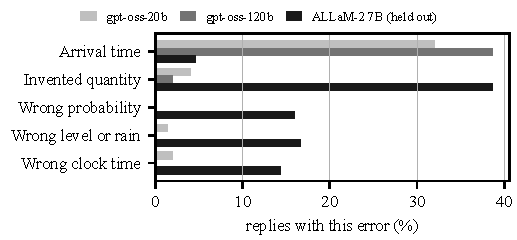
\includegraphics[width=\columnwidth]{fig_errtypes.pdf}
\caption{Kinds of unsupported numbers in live replies, as a share of each model's replies (reference labels). A reply can contain more than one kind.}
\label{fig:errtypes}
\end{figure}
 The frozen guard caught \HoVtwoRec\% of them and missed \HoVtwoMiss{}, against \HoDepRec\% for the deployed guard. Its false-rejection rate, however, rose from \DevVtwoFpr\% to \HoVtwoFpr\% (\HoVtwoFp{} replies). Every one of these was a procedural number that the development models never wrote, such as ``Team 1'', ``Mission 4'' or ``level 2 alert''. The deployed guard rejected fewer grounded replies (\HoDepFpr\%), and the first typed guard more (\HoTypFpr\%). Table~\ref{tab:example} shows four real excerpts.

\begin{table}[t]
\caption{Excerpts from held-out replies and the verdict of each check}
\label{tab:example}
\centering
\footnotesize
\setlength{\tabcolsep}{2.4pt}
\begin{tabular}{>{\raggedright\arraybackslash}p{4.05cm}cccc}
\toprule
Excerpt (content) & Label & $\Gamma$ & $\Gamma_{\mathrm{T}}$ & $\Gamma_{\mathrm{T}}^{(2)}$\\
\midrule
``probability of flooding is at 34.3\%'' (state value) & yes & pass & pass & pass\\
``begun flooding with 134 affected'' (head-count) & no & \textbf{rej.} & \textbf{rej.} & \textbf{rej.}\\
``NDRF teams is 20:59 IST'' (arrival time) & no & \textbf{rej.} & \textbf{rej.} & \textbf{rej.}\\
``Team 1 (Rescue) will head to'' (label) & yes & \textbf{rej.} & \textbf{rej.} & \textbf{rej.}\\
\bottomrule
\multicolumn{5}{l}{\scriptsize Label: supported by the state (reference protocol).}\\
\multicolumn{5}{l}{\scriptsize rej.: the reply is replaced by a template.}\\
\end{tabular}
\end{table}

Two lessons follow. First, a guard that is perfect on the replies used to build it can still fail on a new model, so a guard needs a held-out test just as a classifier does. Second, the errors of a typed guard on new traffic were safe ones: it replaced a correct message by a template, which costs some wording, while it let through only one unsupported number. Checking one reply with $\Gamma_{\mathrm{T}}^{(2)}$ took \VtwoUs~$\mu$s on average on a laptop, a negligible delay for a radio message.

\subsection{Dual-Model Gate}
On the prototype's rainfall sweep (\DualN{} settings) the gate held dispatch in \DualHold\% of settings, including \DualBothHeld\% of those where both models already exceeded $\tau_a$; the mean gap between the models (\DualMeanGap) exceeded $\delta$ itself. Table~\ref{tab:calib} explains why with held-out data. The XGBoost policy model was poorly calibrated (ECE \EceXgb, against \EceRf{} for the Random Forest; Fig.~\ref{fig:rel}): above $\tau_a$ it predicted \XgbHighConf{} on average where floods occurred at a rate of \XgbHighFreq, so the two models differ systematically. Disagreement still carried information: on the \CalTest{} held-out rows the deployed gate held \GateDepHold\% of cases, and the policy model was wrong on \GateDepErrHeld\% of held cases against \GateDepErrRel\% of released ones. The straddle rule alone held only \GateStHold\% of cases, never one in which both models recommended action, and the policy model was wrong on \GateStErrHeld\% of them. The tolerance set from training data alone, $\delta_{95}=\DeltaCv$, behaved similarly and is close to the value at which the sweep stopped holding cases on which both models agreed. Isotonic calibration on the training split lowered ECE to \EceCalXgb{} and \EceCalRf{} and the hold rate of the deployed rule to \GateCalHold\%.

\begin{figure}[t]
\centering
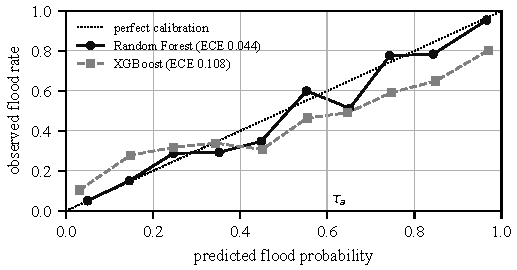
\includegraphics[width=\columnwidth]{fig_reliability.pdf}
\caption{Reliability of the two deployed classifiers on the \CalTest{} held-out rows (bins with at least 10 rows). Points below the diagonal are over-confident.}
\label{fig:rel}
\end{figure}

\begin{table}[t]
\caption{Gate (\ref{eq:dual}) on \CalTest{} held-out rows of the classifiers' split}
\label{tab:calib}
\centering
\footnotesize
\setlength{\tabcolsep}{2.6pt}
\begin{tabular}{lcccc}
\toprule
 & Held & Held, both & \multicolumn{2}{c}{Error \%}\\
Rule & \% & $\ge\tau_a$ \% & held & released\\
\midrule
$\delta=0.15$ (deployed) & 26.9 & 29.1 & 37.1 & 20.3\\
$\delta_{95}=0.28$ (train CV) & 9.1 & 2.2 & 48.2 & 22.5\\
straddle only & 7.6 & 0.0 & 52.2 & 22.6\\
isotonic, $\delta=0.15$ & 10.5 & 7.0 & 39.6 & 22.4\\
\bottomrule
\multicolumn{5}{l}{\scriptsize Flood rate in the test rows: \CalPos\%. Error: of the policy model.}\\
\multicolumn{5}{l}{\scriptsize isotonic: both models calibrated on the training split.}\\
\end{tabular}
\end{table}

\section{Discussion and Limitations}
The results support a division of labour, and they locate its weak points in the glue between components. A dispatch step bypassed a verified policy, a gate tolerance was never related to the calibration of the models it compares, and an untyped guard treated every number as interchangeable. None of these showed up when components were tested one at a time. For safety-critical agentic systems this argues for checking properties on the full path from observation to action and for keeping the components with authority to act few and small. The live study changes the picture from injected errors, and the held-out model changes it again. The two development models rarely corrupted the facts they were given; they \emph{added} quantities the state does not contain, above all arrival times. The held-out model added head-counts and rates and also misquoted the facts themselves. Which errors appear depends on the model, so a check designed around one model's habits has to be tested again on the next one. A check that only asks whether a number exists in the fact sheet is weakest on exactly that error, while a typed check needs rules for the procedural numbers that real traffic contains. A fail-closed fallback also hides what it absorbs: while we prepared this study, retired API models and a token budget too small for reasoning models had silently sent every reply to the template.

Several limits apply. The live study covers three open-weight models from two families, one prompt and \LiveStates{} states; the held-out model already erred differently from the others, and further models will too. Reference labels were assigned with a written protocol and checked by reading, by one annotator; the distinction between claims and procedural numbers is a judgement, and we release the protocol and labels so that it can be re-examined. River and barrage values were sampled from operating ranges, not recorded events. The guards check numbers only, so the qualitative over-claims above, a wrong place or a wrong instruction would pass. The policy check proves properties of (\ref{eq:policy}), not of the health checks that feed it, and the composed check covers the dispatch rule on a grid rather than a proof of the asynchronous pipeline. The calibration study uses the classifiers' random split of flood events; a time-aware split may give different numbers. No officer has used the system in an exercise.

For a deployment we draw three practical rules from these results. Ask the narrator not to produce arrival times, counts or unit labels, since the state contains none of them. Measure the template-fallback rate per model, because it is the only sign of a guard that has started to reject correct traffic. And re-run a labelled held-out test whenever the model behind the API changes, as providers retire and replace models without notice.

Future work will deploy the typed guard with explicit procedural slots, forbid arrival times in the prompt and the guard, replace the gap tolerance with the straddle rule, and run a table-top exercise with emergency officers.

\section{Conclusion}
We presented a flood-response architecture in which deterministic agents hold every decision and an LLM only narrates. Exhaustive testing verified the decision policy, yet the dispatch path did not consult it in \EtoEViolBefore{} cases; after a one-line fix, the composed check found no violation in \EtoECases{} cases. In \LiveN{} real replies of two open-weight LLMs, \LiveUnsupPct\% stated an unsupported number, mostly invented arrival times; the deployed guard caught \LiveDepRec\% of them and a typed guard \LiveTypRec\%. A revised guard kept \HoVtwoRec\% recall on a held-out model but rejected \HoVtwoFpr\% of correct replies, while an LLM judge caught all it checked but missed one-digit errors that the typed guard caught. On held-out data, model disagreement did signal error, and the straddle rule held a quarter as many cases as the deployed gate while flagging errors more sharply. LLM narration can serve an operations net only if it stays outside the decision path and is checked, with types, against the state it describes.

\section*{Acknowledgment}
The authors thank the INDOFLOODS dataset authors and Open-Meteo for openly available data.
In line with the IEEE policy on AI-generated content, the authors disclose that Claude (Anthropic) was used to help edit and restructure the text of all sections and to draft the experiment and plotting scripts. All experiments use the authors' own software and can be reproduced with fixed seeds; the live LLM replies are stored with the scripts. The authors checked every number, claim and reference and take full responsibility for the content.

\balance
\begin{thebibliography}{00}
\bibitem{Ji2023} Z. Ji \textit{et al.}, ``Survey of hallucination in natural language generation,'' \textit{ACM Comput. Surv.}, vol. 55, no. 12, Art. no. 248, 2023, doi: 10.1145/3571730.
\bibitem{Yao2023} S. Yao \textit{et al.}, ``ReAct: Synergizing reasoning and acting in language models,'' in \textit{Proc. Int. Conf. Learn. Represent. (ICLR)}, 2023.
\bibitem{Schick2023} T. Schick \textit{et al.}, ``Toolformer: Language models can teach themselves to use tools,'' in \textit{Adv. Neural Inf. Process. Syst. 36}, 2023.
\bibitem{Wu2024} Q. Wu \textit{et al.}, ``AutoGen: Enabling next-gen LLM applications via multi-agent conversation,'' in \textit{Proc. Conf. Lang. Model. (COLM)}, 2024.
\bibitem{Parasuraman2000} R. Parasuraman, T. B. Sheridan, and C. D. Wickens, ``A model for types and levels of human interaction with automation,'' \textit{IEEE Trans. Syst., Man, Cybern. A, Syst. Humans}, vol. 30, no. 3, pp. 286--297, 2000, doi: 10.1109/3468.844354.
\bibitem{Leveson2011} N. G. Leveson, \textit{Engineering a Safer World: Systems Thinking Applied to Safety}. Cambridge, MA, USA: MIT Press, 2011.
\bibitem{Zheng2023} L. Zheng \textit{et al.}, ``Judging LLM-as-a-judge with MT-Bench and Chatbot Arena,'' in \textit{Adv. Neural Inf. Process. Syst. 36 (Datasets Benchmarks Track)}, 2023.
\bibitem{Wooldridge1995} M. Wooldridge and N. R. Jennings, ``Intelligent agents: Theory and practice,'' \textit{Knowl. Eng. Rev.}, vol. 10, no. 2, pp. 115--152, 1995, doi: 10.1017/S0269888900008122.
\bibitem{Kitano1999} H. Kitano \textit{et al.}, ``RoboCup Rescue: Search and rescue in large-scale disasters as a domain for autonomous agents research,'' in \textit{Proc. IEEE Int. Conf. Syst., Man, Cybern. (SMC)}, Tokyo, Japan, 1999, pp. 739--743, doi: 10.1109/ICSMC.1999.816643.
\bibitem{WangL2024} L. Wang \textit{et al.}, ``A survey on large language model based autonomous agents,'' \textit{Front. Comput. Sci.}, vol. 18, no. 6, Art. no. 186345, 2024, doi: 10.1007/s11704-024-40231-1.
\bibitem{Lewis2020} P. Lewis \textit{et al.}, ``Retrieval-augmented generation for knowledge-intensive NLP tasks,'' in \textit{Adv. Neural Inf. Process. Syst. 33}, 2020, pp. 9459--9474.
\bibitem{Min2023} S. Min \textit{et al.}, ``FActScore: Fine-grained atomic evaluation of factual precision in long form text generation,'' in \textit{Proc. Conf. Empir. Methods Nat. Lang. Process. (EMNLP)}, 2023, pp. 12076--12100, doi: 10.18653/v1/2023.emnlp-main.741.
\bibitem{Manakul2023} P. Manakul, A. Liusie, and M. J. F. Gales, ``SelfCheckGPT: Zero-resource black-box hallucination detection for generative large language models,'' in \textit{Proc. Conf. Empir. Methods Nat. Lang. Process. (EMNLP)}, 2023, pp. 9004--9017, doi: 10.18653/v1/2023.emnlp-main.557.
\bibitem{Dhuliawala2024} S. Dhuliawala \textit{et al.}, ``Chain-of-verification reduces hallucination in large language models,'' in \textit{Findings Assoc. Comput. Linguist. (ACL)}, 2024, pp. 3563--3578, doi: 10.18653/v1/2024.findings-acl.212.
\bibitem{Rebedea2023} T. Rebedea, R. Dinu, M. N. Sreedhar, C. Parisien, and J. Cohen, ``NeMo Guardrails: A toolkit for controllable and safe LLM applications with programmable rails,'' in \textit{Proc. Conf. Empir. Methods Nat. Lang. Process.: Syst. Demonstrations}, 2023, pp. 431--445, doi: 10.18653/v1/2023.emnlp-demo.40.
\bibitem{Zhang2025} Y. Zhang, S. Y. Emma, A. L. J. En, and J. S. Dong, ``RvLLM: LLM runtime verification with domain knowledge,'' in \textit{Adv. Neural Inf. Process. Syst. 38}, 2025.
\bibitem{WangH2026} H. Wang, C. M. Poskitt, and J. Sun, ``AgentSpec: Customizable runtime enforcement for safe and reliable LLM agents,'' in \textit{Proc. IEEE/ACM 48th Int. Conf. Softw. Eng. (ICSE)}, 2026, pp. 2938--2950, doi: 10.1145/3744916.3764546.
\bibitem{Alshiekh2018} M. Alshiekh, R. Bloem, R. Ehlers, B. K\"{o}nighofer, S. Niekum, and U. Topcu, ``Safe reinforcement learning via shielding,'' in \textit{Proc. AAAI Conf. Artif. Intell.}, vol. 32, no. 1, 2018, pp. 2669--2678, doi: 10.1609/aaai.v32i1.11797.
\bibitem{Dietterich2000} T. G. Dietterich, ``Ensemble methods in machine learning,'' in \textit{Multiple Classifier Systems} (LNCS, vol. 1857). Berlin, Germany: Springer, 2000, pp. 1--15, doi: 10.1007/3-540-45014-9\_1.
\bibitem{Lakshminarayanan2017} B. Lakshminarayanan, A. Pritzel, and C. Blundell, ``Simple and scalable predictive uncertainty estimation using deep ensembles,'' in \textit{Adv. Neural Inf. Process. Syst. 30}, 2017, pp. 6402--6413.
\bibitem{Breiman2001} L. Breiman, ``Random forests,'' \textit{Mach. Learn.}, vol. 45, no. 1, pp. 5--32, 2001, doi: 10.1023/A:1010933404324.
\bibitem{Chen2016} T. Chen and C. Guestrin, ``XGBoost: A scalable tree boosting system,'' in \textit{Proc. 22nd ACM SIGKDD Int. Conf. Knowl. Discov. Data Min.}, 2016, pp. 785--794, doi: 10.1145/2939672.2939785.
\end{thebibliography}

\end{document}
